\documentclass[10pt,twocolumn]{article}

\usepackage{times}
\usepackage{fullpage}
\usepackage{graphicx}
\usepackage{epstopdf}

\begin{document}

\title{Efficient Virtualization on Embedded Power Architecture}
\author{}
\date{}
\maketitle
\thispagestyle{empty}

\maketitle
\begin{abstract}
  Power Architecture is popular and widespread on embedded systems, and such
  platforms are
  increasingly
  being used to run virtual machines\cite{XXX}. While the Power architecture meets the
  Popek-and-Goldberg virtualization requirements for traditional trap-and-emulate
  style virtualization, the performance overhead of virtualization remains high.
  For example, workloads exhibiting a large amount of kernel activity typically
  show 3-5x slowdowns over bare-metal.

  Recent additions to the Linux kernel contain guest and host side paravirtual
  extensions for Power Architecture. While these extensions improve performance significantly, they
  are guest-intrusive, non-portable and cover only a subset of all possible
  virtualization optimizations.

  We present a set of host-side optimizations that achieve comparable
  or better performance
  than the aforementioned paravirtual extensions, yet being guest-agnostic. Our
  prototype implementation based on Linux/KVM can run (largely) unmodified, untrusted
  Power Architecture guests at near native performance for almost all workloads. The only
  guest modification required is to include a device driver for our virtual
  device which creates a shared address space between the guest and the host.
  After our modifications, KVM can boot a Linux guest 3x faster. Our solution
  provides equivalent performance (sometimes outperforming by up to XX\%) to
  the paravirtual approach previously included in the Linux kernel, without
  being guest-specific.
\end{abstract}
\section{Introduction}
Power Architecture is a dominant platform for embedded devices for it's
favourable power/performance characteristics. Virtualization on these platforms is
compelling for several applications\cite{XXX}. While newer Power platforms
have explicit support for efficient virtualization\cite{XXX}, a majority of
prevalent embedded devices run on older (and cheaper) Power platforms that use
traditional trap-and-emulate style virtualization\cite{XXX}. Hence, efficient
virtualization is highly desirable on these platforms.

The current virtualization approach on Power Architecture uses traditional
trap-and-emulate. The guest operating system is run unprivileged, causing each
execution of a privileged
operation to exit into the hypervisor. For guest workloads executing a large number
of priviliged instructions, these exits are a major performance
bottleneck. Table~\ref{tab:kvm_performance} lists the performance of vanilla Linux/KVM
on some common workloads.

The poor performance of simple trap-and-emulate style virtualization has led to
the inclusion of paravirtual extensions to the Linux kernel on both
guest and host sides. The paravirtual extension in the guest rewrites the guest kernel
code at startup time to replace most privileged instructions with
hypervisor-aware unprivileged counterparts. The unprivileged version of an
otherwise privileged guest operation typically reads or writes to a hypervisor-visible
shared address, thus providing an efficient mechanism for a {\em hypercall}.
On the host side, a mechanism is provided to setup a shared address space with the guest,
and to execute hypercalls on behalf of the guest. The third column in
Table~\ref{tab:kvm_performance} lists the performance of Linux/KVM with paravirtual
extensions. In this case, both guest and host are running Linux with their respective
paravirtual extensions. The performance improves significantly for many common
workloads.

There are some shortcomings to the paravirtual approach. Firstly, extensive guest
modifications are required making it highly specific to Linux. A different
guest OS, or subsequent updates to Linux, require substantial software
development and maintenance effort. Secondly, all guest
privileged instructions are rewritten only at kernel load time. Hence,
optimizations are
not possible for privileged code running as loadable kernel modules. This
approach will also break in the presence of dynamically generated code, and makes
assumptions about the programming discipline in Linux. For example, this approach
assumes that Linux kernel will never read it's own code as data. Violation of
these programming disciplines in future Linux versions, can render these paravirtual
extensions unusable.

We propose a host-side adaptive binary translation mechanism to optimize guest
privileged instructions at runtime. Our approach requires almost no guest modifications
(except a virtual device driver to setup shared address space), and achieves
comparable or better performance than paravirtual approaches. Because we translate
guest code at runtime (and not at kernel startup time, as done in the paravirtual
approach), we
can optimize code in both the main kernel and the loadable modules. Our approach also
does not assume anything about the guest, and ports seamlessly to different
guests or different versions of the same guest.
The last column in Table~\ref{tab:kvm_performance} summarizes the performance results of
our host-side binary translation approach. In the rest of the paper, we discuss
our approach and the various optimizations we used to achieve these results.

We translate the guest's instructions {\em in situ} (in-place), thus modifying the guest's
address space. This is in contrast with previous full binary translation approaches
that translate the entire guest
code (e.g., VMware's x86-based VMM\cite{agesen:comparison}). Our approach is much
simpler and thus incurs significantly less overhead. For example, a full binary
translator requires a table lookup on every indirect branch (e.g., function return) which
can result in high overheads on many common workloads. In contrast, our lightweight
binary translator simply translates the privileged instructions and allows all other
instructions to run natively.

There are many interesting problems we solved during the development of our
binary translation solution. 
Firstly, while modifying guest instructions, we must ensure correctness in presence
of arbitrary jumps to any instruction. We do this by relying on the fixed-length
word-aligned nature of Power Architecture instructions. Guest instructions
that need to be translated to multiple host instructions for correct emulation, are
handled by jumping to code fragments in a VMM-managed translation cache (full
details in Section~\ref{sec:binarytranslation}.

Secondly, modifying guest instructions in-place requires the VMM to maintain guest
fidelity if the guest reads/writes it's own code. We maintain fidelity by 
marking the pages containing the modified instructions {\em execute-only}. This
causes the hardware to trap into the VMM on any guest read/write access to the
modified page.

Thirdly, marking the modified pages execute-only can result in a large number of
page faults, especially due to false sharing. The problem is particularly
severe in the embedded Power Architecture which has a software-managed TLB with
a small number of variable-sized TLB entries. We found that our modifications to
the guest instructions resulted in a large number of such page faults, thus causing
another source of performance degradation. We discuss two schemes to correctly
and efficiently deal with this problem (Section~\ref{sec:reducing_page_faults}).

We rely on Power Architecture features to implement our
scheme correctly and efficiently. For example, we use
Power Architecture's {\tt read-write-execute} page protection bits to ensure guest
fidelity. In contrast, the x86 architecture provides only {\tt read-only} and
{\tt no-execute} (NX) bits, which are less powerful, and insufficient
to implement our scheme. As another
example, we use Power
Architecture's fixed-length aligned instruction encoding to be able to
perform in-place binary translation correctly. Such ideas cannot be used
on x86 where the guest could potentially jump to the middle of an instruction.
We find that these subtle
differences in different architectures greatly impact VMM design. Just like some
of our aforementioned ideas are not applicable to
x86, some of the ideas in VMware's x86-based binary translator
are not applicable to Power Architecture. For example, VMware's binary translator
relies on x86's segmentation hardware but Power Architecture does not
support segmentation.

In summary, this paper presents an efficient host-side optimization solution for
Power virtualization. Our approach is based on in-place binary translation.
The only guest-side modification required by our solution is a virtual
device driver to map a shared address space between the guest and the host.
We can run untrusted guests and preserve guest fidelity by implementing efficient
tracing mechanisms.
The paper is organized as
follows. Section~\ref{sec:performance_char} characterizes the performance of
KVM on Power Architecture and discusses the typical sources of overhead.
We discuss the setup of shared address space between the guest and host
in Section~\ref{sec:sharedspace}.
Section~\ref{sec:bintrans} discusses our in-place binary translation approach.
Section~\ref{sec:tracing} discusses our tracing mechanism to maintain guest fidelity.
We discuss the performance results obtained by
implementing these mechanisms in Section~\ref{sec:results1}. Section~\ref{sec:tracingopt}
discusses further optimizations to make the tracing mechanism more efficient.
Section~\ref{sec:results2} presents our final performance results, and
Section~\ref{sec:conclusion} concludes.

\section{Performance Characterization of KVM on Power Architecture}
\label{sec:performance_char}
We perform our experiments on Linux/KVM version XXX running on an
embedded Power Architecture processor from Freescale used in network
routing.
Table~\ref{tab:kvm_performance} shows the timing characteristics of
different benchmarks running on KVM on Power Architecture. The
overhead is due to VM-exits caused by execution of priviliged instructions
at unprivileged level. Table~\ref{tab:priv_opcodes} lists the privileged
opcodes and briefly explains their semantics.
Table~\ref{tab:opcode_time_fraction} shows
the different benchmarks and the fraction of time spent in handling
exits due to each opcode respectively. The analysis confirms that a
majority of the time overhead is being spent in handling VM-exits due
to privileged opcodes.

We next profile the number of distinct program counter (PC) values that
cause exits. Figure~\ref{fig:pc_profile} shows a histogram on the number
of distinct PC values and the frequency of exits on them. These results
confirm that most of the exits in almost all our benchmarks are caused
by a small number of distinct PC values. Intuitively, the privileged
instructions on the hot code paths are the biggest culprits.

The breakdown of performance results in Table~\ref{tab:opcode_time_fraction}
and Figure~\ref{fig:pc_profile} confirms that optimization of these
few opcodes occuring at a few distinct PC values is likely to produce
significant runtime improvements. The next section discusses our
optimization solution based on in-place binary translation.

\begin{table}[!b]
\centering
\caption{Sources of VM Exits}
     \begin{tabular}{|l | p{5cm} |} \hline
       Opcode \verb, , & Description \\ \hline
       MFMSR & Move from machine state register \\ \hline
       MTMSR & Move to machine state register \\\hline
	   MFSPR & Move from special purpose register \\\hline
	   MTSPR & Move to special purpose register \\\hline
	   WRTEE(I) & Write MSR External Enable  \\\hline
	   RFI & Return from interrupt \\\hline
	   $[$DI$]$TLBREAL & guest tlb does not have a mapping for the address\\\hline
	   $[$DI$]$TLBVIRT & tlb fault due to virtualization. Host tlb does not have a mapping which is present in guest tlb \\    \hline
   	   DSI & Exits due to access privilege \\\hline

     \end{tabular}
\label{tab:priv_opcodes}
\end{table}

\begin{figure}[!htb]
\centering

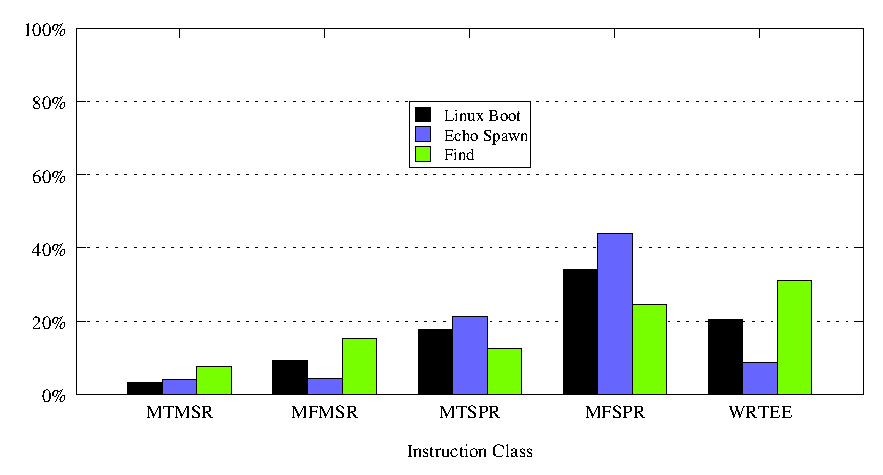
\includegraphics[scale=0.5]{exit_count.eps}
\caption{\% of Total exits}
\label{fig:opcode_ti_fraction}
\end{figure}

\begin{figure}[!htb]
\centering

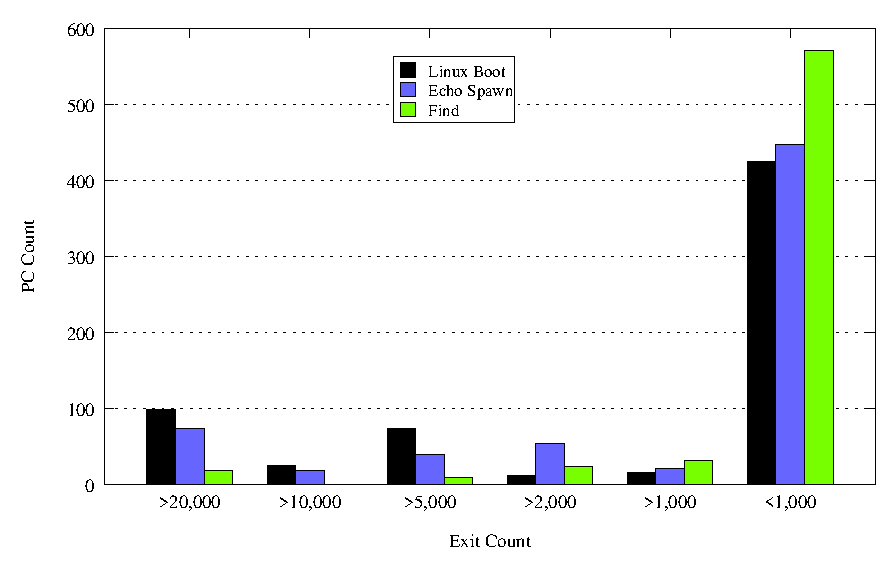
\includegraphics[scale=0.5]{pc_count.eps}
\caption{PC frequency}
\label{fig:pc_profile}
\end{figure}

\begin{table*}
\centering
\caption{Performance comparison}
      \begin{tabular}{|l| l|p{5cm} | c c c c|} \hline
	        S.No.\verb, ,&  Benchmark\verb, ,& Description  & Bare-metal \verb, ,& Base KVM \verb, , & LABT KVM \verb, ,& PV KVM \\ \hline

     &&& \multicolumn{4}{c|}{ Running Time in $sec$}\\\cline {4-7}  
      1&  Linux Boot& linux boot & 6.5	& 30.03	& 12.24	& 11.79 \\ \hline
      2& Echo Spawn	& Spawning a large number of echo processes&1.4	& 21.34 &	7.26 &	6.5 \\\hline
      3& Find	& find / -name temp & 0.39	& 1.89	& 0.71	& 0.67 \\ \cline{4-7}
	   &&& \multicolumn{4}{c|}{Latency in $msec$}\\  \cline{4-7}

  4& syscall	& &	0.001	&	0.021	&	0.004	&	0.004	\\\hline
5&stat	&&	0.003	&	0.033	&	0.007	&	0.006	\\\hline
6&fstat	&&	0.001	&	0.021	&	0.005	&	0.004	\\\hline
7&open/close:	&&	0.007	&	0.067	&	0.015	&	0.013	\\\hline
8&sig hndl	&&	0.001	&	0.024	&	0.004	&	0.004	\\\hline
9&pipe 	&&	0.015	&	0.165	&	0.035	&	0.033	\\\hline
10&fork	&&	1.084	&	6.641	&	2.061	&	1.64	\\\hline
11&exec	&&	3.065	&	20.543	&	7.533	&	6.254	\\\hline
12&sh	&&	6.645	&	45.164	&	16.327	&	13.842	\\\hline

        \hline
      \end{tabular}
\label{tab:lpGMKLsmall}
\end{table*} 


\begin{table*}
\centering
\caption{Context switch times in $ms$}
      \begin{tabular}{|l | c| c |c |c|} \hline
       Case\verb, ,  & Bare-metal \verb, ,& Base KVM \verb, , & LABT KVM \verb, ,& PV KVM \\ \hline

2p0k	&	0.004	&	0.028	&	0.007	&	0.011	\\ \hline
2p16k	&	0.007	&	0.034	&	0.013	&	0.012	\\ \hline
2p32k	&	0.015	&	0.067	&	0.012	&	0.012	\\ \hline
8p0k	&	0.005	&	0.151	&	0.05	&	0.056	\\ \hline
8p16k	&	0.023	&	0.331	&	0.097	&	0.096	\\ \hline
8p32k	&	0.065	&	0.358	&	0.136	&	0.121	\\ \hline
16p0k	&	0.005	&	0.165	&	0.057	&	0.059	\\ \hline
16p16k	&	0.048	&	0.366	&	0.129	&	0.122	\\ \hline
16p32k	&	0.171	&	0.448	&	0.183	&	0.184	\\ \hline

        \hline
      \end{tabular}
\label{tab:lpGMKLsmall}
\end{table*} 


\begin{table}[!b]
\centering
\caption{Performance of Base KVM}
     \begin{tabular}{lcc} \hline
       Benchmark  & Performance (\% of native) \\ \hline
       Linux Boot & 21.7 \\
       Echo Spawn & 6.4 \\
       Find & ${-}$ \\
       \hline
     \end{tabular}
\label{tab:PerfBase}
\end{table}


\begin{table}[!b]
\centering
\caption{Sources of VM exits for linux boot}
     \begin{tabular}{lcc} \hline
       Instruction class  & Exit count & \% of total exits  \\ \hline
       MFSPR & 4484245 & 33.8  \\
       WRTEE & 2792109 & 21.1  \\
       MTSPR & 2307647 & 17.4  \\
       RFI & 575302 & 9.5 \\
       MTMSR & 413847 & 4.3 \\
       TLBWE & 391813 & 3.1 \\
       DTLBREAL & 247282 & 2.9 \\
       ITLBREAL & 241070 & 1.8 \\
       DTLBVIRT & 198239 & 1.5 \\
       ITLBVIRT & 192046 & 1.4 \\
       \hline
     \end{tabular}
\label{tab:NumExitsBase}
\end{table}

\begin{table}[!b]
\centering
\caption{PCs responsible for VM exits for linux boot}
     \begin{tabular}{lcc} \hline
       Exits count  & PC count & \% of total exits  \\ \hline
       $>$20000 & 93 & 91.9  \\
       $>$10000 & 23 & 3.1  \\
       $>$5000 & 68 & 4.2  \\
       $>$2000 & 12 & 0.3 \\
       $>$1000 & 17 & 0.2 \\
       $<$1000 & 299 & 0.2 \\
       \hline
     \end{tabular}
\label{tab:NumPCBase}
\end{table}
\section{Shared Guest-Hypervisor Address Space}
\label{sec:sharedspace}
Our solution requires setting up a shared address space between the
guest and the hypervisor to store the emulated
data and emulated instructions.
We achieve this by requiring the guest to install a virtual guest
device driver provided by us. This is the
only guest-specific change required by our solution. The virtual
device driver reserves
one page with read/write privileges in guest address space. This page
is used by the hypervisor to maintain
emulated guest registers. The virtual guest device driver also
reserves one page with execute privileges in guest address space.
This page is used by the hypervisor to store the binary translator's
translation cache.

Unlike the parvirtual extensions introduced in Linux, these guest
modifications are small and non-intrusive. Such guest virtual device drivers
can also be implemented for closed-source guests.

The execute-only page reserved in guest address space has a special
constraint. As we explain in the
next section, this page must lie within $\pm$16MB of the
guest kernel's code section, for certain translations to be possible.
Given that most guest kernel code sections are
small (e.g., XXX MB for Linux), this constraint is usually easy to satisfy.

Finally, we note that requiring a guest-side device driver for performance
is a well-accepted virtualization practice. For example, x86-based hypervisors
typically require installation of ``tools'' in the guest for better performance.

\section{In-place Binary Translation}
\label{sec:bintrans}
We implement in-place binary translation by replacing the
privileged instructions
with their emulated counterparts directly
in the guest's address space. Some of the privileged instructions can
be emulated by single instructions. For example, {\tt mfmsr} is translated
to a {\tt load} instruction to the address of the emulated {\tt msr}
register in the shared read/write page. The opcodes which can be
translated to single instructions are XXX.

Other privileged opcodes require emulations which involve multiple instructions.
For such opcodes, we store the emulation code in the translation cache, and
patch the original instruction to branch to it. We call the privileged instruction
that was patched, the {\em patch-site}. The emulation code is terminated
with a branch back to the instruction following the patch-site
(see Figure~\ref{fig:txcache}). Because each patch-site requires a different
terminating branch instruction, a new translation is generated for
each patch-site.

We use Power Architecture's unconditional direct {\tt branch} opcode to jump to the
translation cache from the patch-site. The {\tt branch} opcode specifies a 24-bit
branch offset, with either absolute or relative addressing. This constrains us
to place the emulation code either within a 24-bit distance of the patch-site (i.e.,
$\pm$16MB) or in the top or bottom 16MB of the guest's virtual address
space (see Figure~\ref{fig:branchtargets}). We ensure this by mapping the shared
page containing our translation cache within $\pm$16MB of the kernel's code
section (as also mentioned in Section~\ref{sec:sharedspace}).

We investigated at least two other possibilities to avoid this constraint
on the branch instruction. In our first attempt, we tried placing the
translation cache on a page in the top 16MB of the kernel's virtual address
space. This allows the {\tt branch} opcode to reach the emulation code from
the patch-site using absolute addressing. However, the emulation code needs to
jump back to the instruction following the branch opcode. This jump-back must not
clobber a guest's register as the register could be potentially live. Because
the target of the jump-back can be arbitrary (anywhere in kernel code), we concluded
that there is no way to achieve this by simply using a direct {\tt branch} opcode.

In our second attempt, we tried using the hardware link register {\tt lr} to store
the address
of the jump-back target. We patched the privileged instruction with a {\tt bl}
instruction to the emulation code and terminated our emulation code with a {\tt blr}
instruction. One advantage of this approach is that it is possible to
reuse one emulation code
for multiple patch-sites containing the same privileged instruction (because the
terminating instruction {\tt blr} is now independent of the patch-site). However, in
doing so, we
clobber the {\tt lr} register. We experimentally found that this can cause
guest inconsistencies in Linux as {\tt lr} is often at patch-sites.
We next tried saving/restoring the
{\tt lr} register at the patch-site before/after branching to the emulation code.
To do this, we patched not just the privileged instruction but also 1-2
surrounding instructions (see Figure~\ref{fig:multiple_insns_patching}). The
surrounding instructions are made part of the emulation code to preserve
guest behaviour. This can
be done safely only if the surrounding instructions are not control-flow instructions.
However, this fails if the guest jumps to the middle of our
three-instruction translation. We discarded this approach because in the presence
of indirect branches, the guest can potentially jump to any instruction boundary.

The hypervisor maintains the state of the translation cache in
a hash table indexed by the PC value of current patch-sites. Each hash table
entry stores information like the original contents of the patch-site,
the location of the corresponding emulation code in the shared page, and other
information useful
for cache replacement. We use the FIFO replacement policy for it's simplicity
and high performance.
\section{Maintaining Guest Fidelity through Read/Write Tracing}
\label{sec:tracing}
Changing instructions in the guest address space can cause
inconsistencies if the guest tries to read or write it's own code.
For this reason, we protect the pages containing patch-sites with hardware
page-protection bits. Embedded Power Architecture provides three {\tt rwx}
protection bits per page. Using these bits, we mark a guest page containing a patch-site
execute only, by setting {\tt r} and {\tt w} bits to 0 and {\tt x} bit to 1.
Any execution of an instruction on this page proceeds uninterrupted
but any read or write access causes a VM exit (page fault).
On a page fault, the hypervisor
emulates the faulting instruction in software. We call this
method memory read/write tracing (similar to VMware's memory tracing
on x86\cite{agesen:comparison}).

For tracing, we implemented software emulations of memory instructions in KVM.
For read instructions, we simply return the original contents of the memory
address in the appropriate destination
operand. The original contents may be obtained either from the present guest
page (if the address does not intersect with a patch-site) or from the hypervisor's
hash table (if the address matches a patch-site) or both.
For write instructions, if the memory address (and length) intersects with a patch-site,
we invalidate and free the corresponding translation cache
entry and replace the guest page with it's original contents before
restarting the instruction. If the memory address does not intersect with a patch
site, we simply return the corresponding contents of guest's memory in the destination
operand.

The overhead of read/write tracing depends on the number of accesses by the guest
to it's pages containing kernel code. For a Linux guest, we found that this overhead
can be quite significant. For example, booting guest Linux can result in
up to XXX page faults due to read/write tracing causing XXX\% performance overhead.
We present detailed experiments to measure this overhead in Section~\ref{sec:results}.

We found that the large number of exits due to read/write tracing were primarily
due to false sharing. Typically, guest kernel data resides on the same page as
guest kernel code, which causes a large number of VM exits. The problem is
worse on embedded Power Architecture due to the presence of {\em huge} pages.
Power Architecture (embedded versions) typically have small software-managed
TLBs with variable-sized pages. Operating systems typically use huge pages to
minimize the number of TLB misses, which exacerbates false sharing problems for
our optimizations.

We implement two mechanisms to offset this tracing overhead. Our first mechanism
adaptively resizes the guest's TLB entries. Our second mechanism optimizes page faults
caused by read accesses (which is the common case) by making a copy of
the read-only data, and translating the read instructions
to access the copied data (instead of the original). The copied data is placed on
a separate page from the patch-sites to avoid tracing page faults. We discuss
both optimizations below.

\subsection{Adaptive TLB splitting/merging}

\subsection{Optimization of DSI reads} - explaination - tracing of root cause by studying results of nanobenchmark syscall - comparison of results with DM-read



\begin{table}[!b]
\centering
\caption{Performance improvement for LABT}
     \begin{tabular}{lcc} \hline
       Benchmark  & Time & Improvement( \% over Base)  \\ \hline
       Linux Boot & 13.1 & 129  \\
       Echo Spawn & 8.2 & 166  \\
       Find & - & -  \\
       \hline
     \end{tabular}
\label{tab:ExpWithout1}
\end{table}

\begin{table}[!b]
\centering
\caption{Performance improvement for LABT}
     \begin{tabular}{lcc} \hline
       Benchmark  & Time & Improvement( \% over Base)  \\ \hline
       Linux Boot & 13.1 & 129  \\
       Echo Spawn & 8.2 & 166  \\
       Find & - & -  \\
       \hline
     \end{tabular}
\label{tab:ExpWithout2}
\end{table}


Discuss the sources of overhead, and TLB thrashing.

\section{Experimental Results}
\label{sec:results2}
Compare with base KVM, paravirtual, and baremetal. Discuss sources of overhead. Discuss
why performance has improved.

\section{Discussion}
\subsection{Multiprocessors}
\subsection{Comparison with Full Binary Translation}
\section{Conclusion}

\bibliography{millirollbacks}
\bibliographystyle{abbrv}

\end{document}
